\documentclass[a4paper, 10pt, twocolumn]{article}
 
%%%%%%%%%%%%%%%%%%%%%%%%%%%%%%%%%%%%%%%%%%%%%%%%%%%%%%%%%%%%%%%%%%%%%%%%%%%%%%
% additional packages 
%\usepackage[dvips]{graphicx}		% optional for graphics
\usepackage{graphicx}		% optional for graphics
\usepackage{tabularx}						% optional for tables
\usepackage{multirow}						% optional for tables
\usepackage{url}								% optional for internet links
\usepackage[ansinew]{inputenc}
\usepackage[small,bf]{caption} 	% for the captions below figures and tables
\usepackage{parskip}
\usepackage{titlesec}
\usepackage{amsmath}						% essential for equations
\usepackage{abstract}
\usepackage{xcolor}							%%bmr - Schriftfarbe
\usepackage{fancyhdr}						%%bmr - Kopf- und Fusszeilen
\usepackage{lipsum}
\usepackage[pdftex, hidelinks]{hyperref}		%%Dokumenteneigenschaften
\usepackage[english]{babel}			%% English- erweiterte Silbentrennung und �bersetzung von Begriffen
%\usepackage{cite} 							%% erlaubt Einbindung von bibrefs
\usepackage{ragged2e}						%% Flattersa
\usepackage{csquotes}
\usepackage[backend=biber,style=ACM-Reference-Format,sorting=none]{biblatex}
\usepackage{textcomp}
%%%%%%%%%%%%%%%%%%%%%%%%%%%%%%%%%%%%%%%%%%%%%%%%%%%%%%%%%%%%%%%%%%%%%%%%%%%%%%

\usepackage{listings}
\usepackage{xcolor}
 
\definecolor{codegreen}{rgb}{0,0.6,0}
\definecolor{codegray}{rgb}{0.5,0.5,0.5}
\definecolor{codepurple}{rgb}{0.58,0,0.82}
\definecolor{backcolour}{rgb}{0.95,0.95,0.92}

\lstdefinelanguage{javascript}{
  keywords={typeof, new, true, false, catch, function, return, null, catch, switch, var, if, in, while, do, else, case, break, let, require, const},
  keywordstyle=\color{blue}\bfseries,
  ndkeywords={class, boolean, throw, implements, import, this, ADD, fs, Matrix},
  ndkeywordstyle=\color{green!50!black}\bfseries,
  identifierstyle=\color{black},
  sensitive=false,
  comment=[l]{//},
  morecomment=[s]{/*}{*/},
  commentstyle=\color{purple}\ttfamily,
  stringstyle=\color{red}\ttfamily,
  morestring=[b]',
  morestring=[b]"
}
 
\lstset{
   language=JavaScript,
   backgroundcolor=\color{white!95!black},
   extendedchars=true,
   basicstyle=\footnotesize\ttfamily,
   showstringspaces=false,
   showspaces=false,
   numbers=left,
   numberstyle=\footnotesize,
   numbersep=9pt,
   tabsize=2,
   breaklines=true,
   showtabs=false,
   captionpos=b
}


\renewcommand{\rmdefault}{ptm}  	% Times New Roman
\newcommand{\citationneeded}[1][]{\textsuperscript{\color{black} [citation needed]}}

\usepackage{pdfpages}

%\bibliographystyle{ACM-Reference-Format}
\bibliography{bibliography.bib}

%%Mit den folgenden Befehlen lassen sich die Dokumenteigenschaften des erstellten PDF Dokuments nach den eigenen W�nschen anpassen:
\hypersetup{pdfauthor = {H. Baumgartner, W. Hoeg, T. Sporer (Ver. 05/2018)},pdftitle = {Template (LaTeX format) for contributions for the ICSA},pdfsubject = {Verband Deutscher Tonmeister (VDT)},pdfkeywords = {keyword 1, keyword 2, etcetera},pdfcreator = {Anwendung},pdfproducer = {PDF erstellt mit}} 
%%Im Adobe Reader lassen diese sich dann mit STRG-D oder "Datei, Eigenschaften�" betrachten.

%%% Bemerkungen: (Unter Verwendung von Elementen einer DAGA-Vorlage)  (Using elements of a DAGA template)

%%% Anpassung fue reviewed Papers

\titleformat{\section}{\normalfont\Large\bfseries}{\thesection.}{11pt}{}
\titleformat{\subsection}{\normalfont\large\bfseries}{\thesubsection.}{2pt}{}
\titleformat{\subsubsection}{\normalfont\normalsize\bfseries}{\thesubsubsection.}{6pt}{}

\setlength{\baselineskip}{0pt}
\setlength{\belowcaptionskip}{-10pt}
\setlength{\parskip}{6pt}

\titlespacing{\section}{0pt}{6pt}{0pt}
\titlespacing{\subsection}{0pt}{3pt}{0pt}
\titlespacing{\subsubsection}{0pt}{0pt}{0pt}

\renewcommand{\abstractnamefont}{\normalfont\large\bfseries}
\renewcommand{\abstracttextfont}{\normalfont\normalsize}

\renewcommand{\thefigure}{\arabic{figure}}
\addto\captionsenglish{%
\renewcommand{\figurename}{Fig.}%
\renewcommand{\tablename}{Tab.}%
}
\renewcommand{\figurename}{Fig.}%
\renewcommand{\tablename}{Tab.}
% Strongly discourage hyphenation
\hyphenpenalty=5000
\tolerance=1000

%%%%%%%%%%%%%%%%%%%%%%%%%%%%%%%%%%%%%%%%%%%%%%%%%%%%%%%%%%%%%%%%%%%%%%%%%%%%%%
\newcolumntype{Y}{>{\centering\arraybackslash}X}	% For tables

%%%%%%%%%%%%%%%%%%%%%%%%%%%%%%%%%%%%%%%%%%%%%%%%%%%%%%%%%%%%%%%%%%%%%%%%%%%%%%
% Definitions page and text marges
\addtolength{\textwidth}{2.1cm}
\addtolength{\topmargin}{-2.7cm}
\addtolength{\oddsidemargin}{-1 cm}
\addtolength{\textheight}{3.8cm}
\setlength{\columnsep}{0.7cm}
\setlength{\voffset}{0.85cm}
\setlength{\headsep}{0.6cm}

%%%%%%%%%%%%%%%%%%%%%%%%%%%%%%%%%%%%%%%%%%%%%%%%%%%%%%%%%%%%%%%%%%%%%%%%%%%%%%
%\pagestyle{empty} 					% no page numbers etc.
\pagestyle{fancy} 
\urlstyle{rm}
%%%%%%%%%%%%%%%%%%%%%%%%%%%%%%%%%%%%%%%%%%%%%%%%%%%%%%%%%%%%%%%%%%%%%%%%%%%%%%
% START OF THE DOCUMENT
%%%%%%%%%%%%%%%%%%%%%%%%%%%%%%%%%%%%%%%%%%%%%%%%%%%%%%%%%%%%%%%%%%%%%%%%%%%%%%
\begin{document}
\fancyhf{} %alle Kopf- und Fusszeilenfelder bereinigen 

\chead{\underline{\sffamily\large\textcolor{gray}{5th International Conference on Spatial Audio ICSA, September 2019}}}
\renewcommand{\headrulewidth}{0pt}
\rhead{}
\renewcommand{\headrulewidth}{0pt}
\rhead{}

\fancyfoot[C]{\footnotesize $^*$ Please note that the papers at ICSA can be published by VDT, in print, online and as PDF download.}

%%%%%%%%%%%%%%%%%%%%%%%%%%%%%%%%%%%%%%%%%%%%%%%%%%%%%%%%%%%%%%%%%%%%%%%%%%%%%%
% FORMATION OF THE TITLE
%%%%%%%%%%%%%%%%%%%%%%%%%%%%%%%%%%%%%%%%%%%%%%%%%%%%%%%%%%%%%%%%%%%%%%%%%%%%%%
\date{}											% no date on page number 1

\title{
%%%spo
\vspace{-5mm}%
\mbox{
\includegraphics[height=4cm]{VDT}}
%
\vspace{7mm}%
%
\begin{center}
\textbf{\Huge Ambisonic Decoder Description (.ADD)}\\
{ Presented  $^*$ by VDT.}
\end{center}
\vspace{10mm}%
 %~\newline
\begin{center}
\textbf\mdseries Developing a new file format for Ambisonics decoding matrices
\end{center}
%
\mbox{}\vspace{-11mm}
%
}

%%%%%%%%%%%%%%%%%%%%%%%%%%%%%%%%%%%%%%%%%%%%%%%%%%%%%%%%%%%%%%%%%%%%%%%%%%%%%%
% Names and affiliation of authors
\author{ %
%
G. Arlauskas, J. Ohland, H. Schaar\\
%
\textit{\large %
University of Applied Sciences Darmstadt, Germany,}\\
\textit{\large Email: \{jonas.ohland, gabriel.p.arlauskas, henning.schaar\}@stud.h-da.de
}\\
%
}
%

\twocolumn[
\maketitle
\thispagestyle{fancy}
%\thispagestyle{empty} 			% no page numbers etc.
%
%%%%%%%%%%%%%%%%%%%%%%%%%%%%%%%%%%%%%%%%%%%%%%%%%%%%%%%%%%%%%%%%%%%%%%%%%%%%%%
% Start of the manuscript
%%%%%%%%%%%%%%%%%%%%%%%%%%%%%%%%%%%%%%%%%%%%%%%%%%%%%%%%%%%%%%%%%%%%%%%%%%%%%%

{\vspace{-3mm}}
\begin{onecolabstract}
{\vspace{3mm}}

Different software solutions have been developed for the calculation and implementation of Ambisonics decoding matrices. The present paper presents and describes a new data file format which can be used as an intermediate between solutions.

Currently available software solutions use particular data conventions causing difficult compatibility and exchangeability. In the present work an open-source toolkit is developed for storing, handling and using Ambisonics decoding matrices. The toolkit includes tools for conversion from common matrix data conventions to the ADD-format and back, calculating decoding matrices, decoding Ambisonics signals and extracting existing matrices from external decoding tools. 

The new ADD-format and toolkit enables increased flexibility in production workflows and eliminates the drawbacks and limitations regarding compatibility between software solutions.

\end{onecolabstract}
{\vspace{8mm}}]

\section{Introduction} \label{sec:introduction}

Spatial audio can be considered as an extension of already established surround sound but in addition to the horizontal plane, the whole three dimensional sound field is described. Ambisonics has been established as a reliable mathematical way to represent the sound field components \autocite{gerzon}. Those components are obtained by encoding a sound source with spherical harmonics.

Spherical harmonics are an infinite set of harmonic functions defined over the surface of a sphere and can be defined as 

\begin{equation}
Y_{\ell}^{m}(\boldsymbol{\vartheta})=N_{\ell,|m|}^{X} P_{\ell}^{|m|}(\cos \theta)\left\{\begin{array}{cc}{\cos (m \phi),} & {\text { for } m \geq 0} \\ {\sin (|m| \phi),} & {\text { for } m<0}\end{array}\right.
\end{equation}

where $\vartheta$ is the angular direction, $P$ is the associated Legendre polynominal of order $\ell$ and index $m$ and $N$ is a normalisation factor obtained by a method X defined either for the Schmidt semi-normalized (SN3D) as

\begin{equation}\label{eq:sn3d}
N_{\ell, |m|}^{\mathrm{SN3D}}=\sqrt{\frac{2-\delta_{m}}{4 \pi}\frac{(\ell-|m|) !}{(\ell+|m|) !}}, \delta_{m}\left\{\begin{array}{ll}{1} & {\text { if } m=0} \\ {0} & {\text { if } m \neq 0}\end{array}\right.
\end{equation}

or for the Fully normalized form (N3D) with an additional factor

\begin{equation}\label{eq:n3d}
    N_{\ell, |m|}^{\mathrm{N} 3 \mathrm{D}}=N_{\ell, |m|}^{\mathrm{SN} 3 \mathrm{D}} \sqrt{2 \ell+1}
\end{equation}

And the encoding of a set of $k$ input signals $g_{l}$ can be expressed as

\begin{equation}
\hat{\boldsymbol{\phi}}=\sum_{k=1}^{\mathrm{K}} \boldsymbol{y}\left(\boldsymbol{\vartheta}_{k}\right) g_{k}
\end{equation}

where


\begin{equation*}
\boldsymbol{y}(\boldsymbol{\vartheta}) :=\left[Y_{0}^{0}(\boldsymbol{\vartheta}), \cdots, Y_{\ell}^{m}(\boldsymbol{\theta}), \cdots\right]^{\mathrm{T}}
\end{equation*}

or in a simplified form as

\begin{equation}
\hat{\boldsymbol{\phi}}=\boldsymbol{\Upsilon} \boldsymbol{g}
\end{equation}

where

\begin{equation*}
\begin{array}{l}{\boldsymbol{g} :=\left[g_{1}, \ldots g_{\mathrm{K}}\right]} \\ {\boldsymbol{\Upsilon} :=\left[y\left(\vartheta_{1}\right), \ldots, y\left(\vartheta_{\mathrm{K}}\right)\right]}\end{array}
\end{equation*}


In most cases the signals $\boldsymbol{s}$ decoded for various loudspeaker setups can be obtained by applying a decoding matrix D

\begin{equation}
    \boldsymbol{s}=\boldsymbol{D} \boldsymbol{\phi}
\end{equation}

Thus decoding an Ambisonics signal, as long as the position of the speakers is constant, is a static operation with low complexity once the matrix has been calculated.

In recent years, numerous approaches have been presented to calculate these matrices. Above all, the approaches differ in their suitability regarding certain speaker systems and playback situations and contents. A good overview of existing approaches, their advantages and disadvantages can be found in \cite{allradepadcomp} and \cite{unstablemmd}

Often these methods are difficult to use in practice. Many of the methods described exist only as implementations for applications tailored to specific fields of research. 

For example, decoding matrices well suited for irregular loudspeaker layouts can be calculated with implementations created for Matlab, such as the EPAD \cite{epad}, CSAD \cite{csad} and AllRAD \cite{allrad} method. However, their use in applications like \textit{ambidecode\texttildelow} \cite{ICSTAmbiPaper} in Max/MSP proves to be difficult. Although both solutions support importing and exporting of decoding matrices as files, the formats are not compatible with each other, even though they both contain the same data.

To overcome compatibility problems like these, we propose the .add format. It should serve as a bridge between different solutions, while still providing enough flexibility to incorporate all common features as well as future developments.

\section{Method} \label{sec:Method}

In order to design such a format, firstly it is recommendable to get an overview of the requirements that meet existing formats. Obviously, it is necessary to describe at least one decoding matrix $ D $ which transfers an incoming set of SH $ \phi $ to the reproduction channels $ s $. Especially interesting though, is the additional data produced by the applications we analyzed, such as e.g. speaker positions, normalization method and output routing.

In this context, we investigated the following solutions:

\paragraph{ambidecode\texttildelow}

ambidecode\texttildelow\ developed in the Zurich Unisersity of Arts \cite{ICSTAmbiOnline} and described in \cite{ICSTAmbiPaper} allows to export and import the internal matrix as an xml file. In addition, the expected normalization of the incoming Ambisonics signal as well as the layout of the speaker system, a gain factor for each output and a set of decoding weights for the ambisonic components can be exported to a separate file.

\paragraph{Ambix decoder}

In addition to the matrix, the configuration files for the ambix decoder \cite{ambiXOnline} also contain information about the expected order of spherical harmonics and a gain factor for the entire matrix.

\paragraph{Compact higher-order Ambisonic Library}

This is a collection of Matlab function for use with higher order ambisonics. \cite{PolarchAmbiLib} None of these functions was explicitly written to generate files but this can be done easily. 

\paragraph{IEM AllRAD decoder}

The AllRAD decoder \cite{IEMFormatOnline} exports not only the matrix and some metadata such as a name and a description but also information about the expected normalization of the ambisonics signal, a desired weighting of Ambisonics components per order, and the layout of the target rendering system. 

\paragraph{IEM Simple Decoder}

The Simple Decoder \cite{IEMFormatOnline} is unable to produce a matrix itself but can read files produced by AllRAD Decoder and use the matrices it contains for ambisonic decoding. In addition, one can specify a subwoofer channel, which will be taken from the matrix output and passed through a high pass filter after decoding. 

\paragraph{Ambilibrium}

Ambilibrium \cite{romanov2018ambilibrium} exports configuration files for the Ambix decoder and the format used by the IEM.

\paragraph{AmbDec}

AmbDec \cite{AmbDecManual} enables the seperation of the Ambisonics signal into two frequency bands and to then decode it with different decoding matrices. Thus, the format produced by the AmbDec offers the possibility to store two matrices, a crossover frequency and a relative gain factor for both frequency bands. Information about the expected normalization, the speaker layout and whether the decoder should make a latency compensation when all speakers are not on the surface of a sphere can also be represented.

\paragraph{ambisonics decoder toolbox}

The ambisonics decoder toolbox \cite{adtpaper} exports ambdec files and configuration files for the ambix decoder. 


%%%%%%%%%%%%%%%%%%%%%%%%%%%%%%%%%%%%%%%%%%%%%%%%%%%%%%%%%%%%%%%%%%%%%%%%%%%%%%
\section{Design} \label{sec:Design}

For the design of the .add format we decided to orient ourselves very close to the design of the configuration files for the IEM plugins. Additionaly, an optional filter stage, optional additional matrices and extended metadata can be saved. All filters and all outputs can be named. An .add file contains a creation date, author information, details about the software it was created with, and a version number. To avoid compatibility problems, a format revision is saved in each file. 

Papers written by Heller et all. \cite{heller2008is, ambifilters} describe the advantages of multiband decoding. For this reason, the .add format supports the basic description of filters applied to the Ambisonics signal before the decoding step with corresponding matrices.

In the description of the filters, we have decided to restrict ourselves to specifying the cut-off frequencies and to leave the filter design to the implementation. However, we encourage the use of phase-matched IIR Filters to preserve uniform frequency response over all directions.

Channel ordering in .add files is done according to the ACN standard, where the channel number can be detemined algorithmically:

\begin{equation}
    ACN=\ell^{2}+\ell+m
\end{equation}

The expected type of normalization is specified with each file and may be either SN3D or N3D as in \eqref{eq:sn3d} and \eqref{eq:n3d} respectively.

As a container format, we chose JSON for a variety of reasons. JSON is widely used and supported by many programming languages. The structure of a JSON object can be represented by native constructs in memory which can be manipulated intuitively. Furthermore, it is human-readable and can be edited with a simple text editor. Compared to XML, JSON strings are favorable regarding data storage space.

\vspace{2mm}
\begin{figure}[htb]
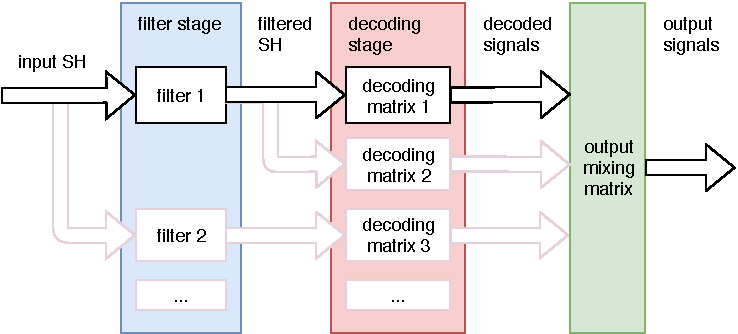
\includegraphics[width=\the\linewidth]{decoding.pdf}
\caption{Schematic representation of an ambisonic decoder that can be described by the .add format.}
\end{figure}
\vspace{2mm}

\section{Implementation} \label{sec:Implementation}

\paragraph{dotaddtool} 
The dotaddtool converts the various formats for storing decoder matrices into .add files and back. This tool enables end users to work with multiple softwares, which have not implemented the .add file format themselves. As such it also serves as an intermediate solution, before .add files have seen widespread adoption.

% \paragraph{dotadd web tool} // vielleicht lieber mal nicht im paper erwähnen?

\paragraph{Decoder Extractor}
Another part of the toolkit is the "dotadd-decoder-extractor" that aims for the particular case when a plugin doesn't allow exporting of decoder matrices.

The tool consists of two VST Plugins using a peer-to-peer inter-process connection which are placed up- and downstream right next to a target decoder plugin. Since a matrix is applied passively in the processing algorithm, sending a signal with a value of 1 through the processor for every channel results in the output being solely the internal decoding matrix used in the plugin. 

Because matrix data can vary depending on e.g. Ambisonics order or channel configuration, it is possible to configure the output signal of the exciter plugin to produce fitting and functional matrix data. The values of the matrix are cached on run-time, recalculated according to configurations specified by the user and lastly exported as an .add-file. The tool can only extract matrices from decoders that do not apply any additional filtering or band-splitting.

\paragraph{Software libraries}

In order to garantee the uniformity of .add files and to facilitate the adaptation, software libraries for the programming languages C ++, Python, JavaScript and Matlab are developed. These allow fast adaptation of existing program infrastructure to the .add format.

Fig. \ref{fig:dotadd} shows a complete example of creating a .add file describing an basic ambisonic decoder with a single output.

\vspace{3mm}
\begin{figure}[htb]
\begin{lstlisting}
    const ADD = require("dotadd.js");
    const fs = require("fs");
    
    let add_file = new ADD()
                .setName("Example Decoder")
                .setAuthor("My Name");
    
    add_file.addMatrix(new ADD.Matrix(
            [[1., 0., 0., 0.]]));
    
    fs.writeFileSync("/output/file.add", 
            add_file.export().serialize());
    \end{lstlisting}
\caption{Creation and export of an .add file in JavaScript for the node.js runtime environment.}\label{fig:dotadd}
\end{figure}
\vspace{2mm}

The Software libraries and tools will be released soon and can be found under \href{https://github.com/smp-3d/dotadd}{https://github.com/smp-3d/dotadd}.

\section{Discussion}\label{sec:Discussion}

Along the history of Ambisonics, developers have contributed to the technology in a gradual manner making the theory practically accessible. Provision of full-fledged toolkits such as SPARTA \cite{SPARTAOnline}, the IEM PluginSuite \cite{IEMPluginsOnline} or the ICST Ambisoncs Externals for Max/MSP \cite{ICSTAmbiOnline} has pushed the limits for widespread usage of Ambisonics technology. However, compatibility issues are still common and prevent industrial use of multi-software solutions. 
As for decoders it still lacks a common ground to improve further according to agreed upon standards. Our proposal is a further step towards a universal workflow with this type of technology. We are optimistic about the outcome and are curious about improvements and open for conversation.



%%%%%%%%%%%%%%%%%%%%%%%%%%%%%%%%%%%%%%%%%%%%%%%%%%%%%%%%%%%%%%%%%%%%%%%%%%%%%%
% REFERENCES
%%%%%%%%%%%%%%%%%%%%%%%%%%%%%%%%%%%%%%%%%%%%%%%%%%%%%%%%%%%%%%%%%%%%%%%%%%%%%%
\renewcommand\refname{}
\section{References}\label{sec:References}

\begingroup
\RaggedRight 		%% Flattersatz

\printbibliography
\endgroup
%%%%%%%%%%%%%%%%%%%%%%%%%%%%%%%%%%%%%%%%%%%%%%%%%%%%%%%%%%%%%%%%%%%%%%%%%%%%%%
\end{document}

%
%Beispiel bibDatei:
%@inproceedings
%{
%Derntl2004Pattern,author= {Derntl, Michael and MotschnigPitrik, Renate},
%title = {Patterns for blended, PersonCentered learning: strategy, concepts,experiences, and evaluation},
%booktitle = {SAC '04: Proceedings of the 2004 ACM symposium on Applied computing},
%year = {2004},
%isbn = {1581138121},
%pages = {916923},
%location = {Nicosia, Cyprus},
%doi = {
%http://doi.acm.org/10.1145/967900.968087
%}

